\clearpage
\section{Experimental validation on a linear axis}
\label{sec:ExperimentalValidation}

The experimental validation reported in the previous \autoref{sec:shaker_test01} and \autoref{sec:shaker_test02} was carried out in a well-controlled environment with a shaker that was able to generate vibrations according to specific references. To further test the framework, a real-world application is considered in this section. The setup consists of a machine equipped with a linear axis, that is used to move a platform. On the moving platform the same accelerometer described in \autoref{tab:adxl335_specifications} has been attached using a custom 3D-printed fixture.

The test consists of defining a set of movements to be actuated by the platform, the accelerometer is used to capture the characteristics of each movement. As done previously, some movement profiles are used for training and others for testing. The position reference is shown in \autoref{fig:etel_profile}, and the parameters of the profiles are resumed in \autoref{tab:etel_profiles}.

\begin{figure}
    \centering
    \todo%\includegraphics{Images/etel/etel_profile.pdf}
    \caption{Position reference for the linear axis test.}
    \label{fig:etel_profile}
\end{figure}

\begin{table}
    \centering
    \caption{Harmonic coefficients for the shaker test.}
    \label{tab:etel_profiles}
    \begin{tabular}{cccc} 
    \toprule
    \textbf{Profile N.} & \textbf{Speed} {[}$\text{m}\text{s}^{-1}$] & \textbf{Acceleration} {[}$\text{m}\text{s}^{-2}$] & \textbf{Jerk} {[}$\text{s}$] \\ 
    \hline
    1 & 0.8 & 6 & 0.02 \\
    2 & 0.4 & 3 & 0.02 \\
    3 & 0.4 & 6 & 0.02 \\
    4 & 0.6 & 8 & 0.02 \\
    \bottomrule
\end{tabular}
\end{table}

\subsection{Training}
To perform the training, a loop has been implemented on the \gls{pc} that manages the axis movements. The script cyclically actuates the axis to follow the reference profile and asks the microcontroller to start the acquisition of the accelerometer data at the beginning of movement. The received features are then stored in a file, and the process is repeated for each profile. The sampling frequency of the microcontroller is 5kHz, for a total of 6000 samples per profile. 

Although not useful for the training, the microcontroller has been set not only to transmit the features to the \gls{pc} but also the time-series, for visualization purposes. The time-series of the training set are shown in \autoref{fig:axis_timeseries}, and the features are shown in \autoref{fig:axis_features}.

In the time-series set it is possible to see some outliers, for example, there is a record in which profile 1 started being actuated by the axis with a delay \gls{wrt} the others. Profile 4, instead, has some outliers due to the axis sometimes overshooting the reference position. These outlier are caused by the axis control, and the investigation about why does it happen is out of the scope of this work. 

The training set contains 100 snapshots for each profile, for a total of 400 snapshots. The K-means model is then trained for $n=5$ clusters, according to the silhouette criterion.

As done previously, the training is performed with the user confirming the correct number of clusters. And updating the model into the microcontroller.

\begin{figure}
    \centering
    \includegraphics{images/LinearMotor/Timeseries.pdf}
    \caption{Timeseries of the training set}
    \label{fig:axis_timeseries}
\end{figure}


\begin{figure}
    \centering
    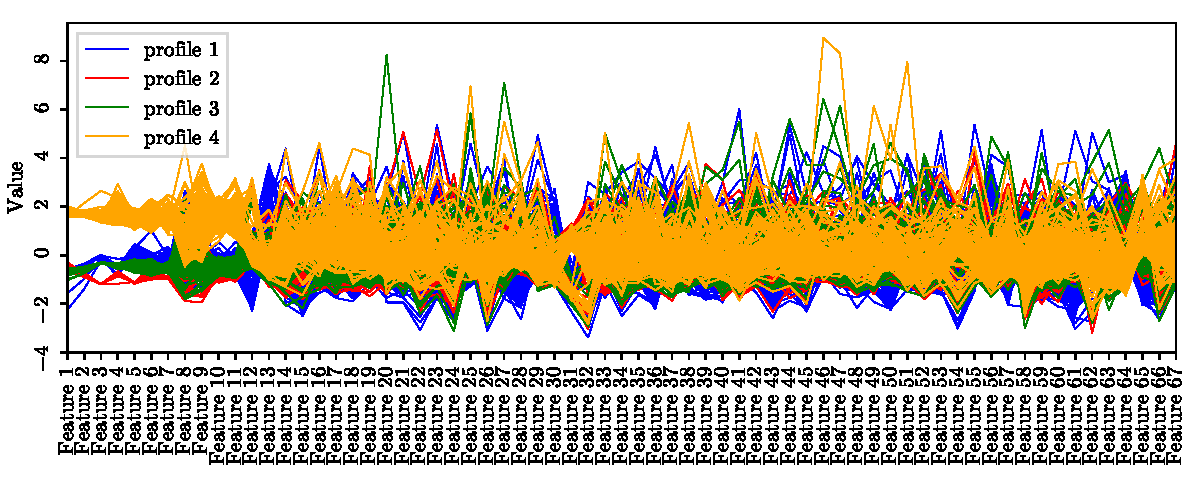
\includegraphics[width=\textwidth]{images/LinearMotor/Features.pdf}
    \caption{features of the training set}
    \label{fig:axis_features}
\end{figure}

\begin{figure}
    \centering
    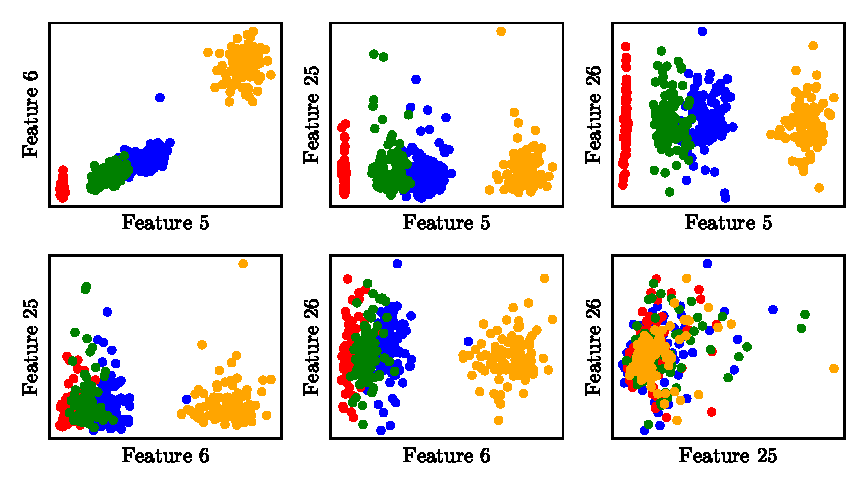
\includegraphics{images/LinearMotor/Scatter.pdf}
    \caption{Visualization of the separation between profiles in the feature space}
    \label{fig:axis_scatter}
\end{figure}


\subsection{Testing}
The microcontroller is then set in \emph{evaluate} mode and the \gls{nd} is performed on a loop that repeats the movement of profile 2. The result of this first model (Model 1) is shown in \autoref{fig:axis_testing}. We can see that the model immediately falsely detects a novelty, despite profile 2 being part of the training set. The figure also shows a clearer view of the evolution of the novelty score, obtained by applying a moving average filter on the last 5 values of the novelty metric.

Let's investigate why this model gives almost all false positive results. Analyzing the features of the training set (\autoref{fig:axis_features}), we can see that the first features, up to $\approx 12$, are grouped by profile, but most of the remaining features are not, this arises the suspect that these features may not be significative of the movement, but maybe just representing noise. This is likely also because the necessary standardization procedure ensures that each feature will have unitary standard deviation, regardless of the magnitude of the feature itself \gls{wrt} the others. This may cause \quoted{noise} features to be amplified in the model. Moreover, it's clear that, being most of the features not significant, the model is not able to distinguish between the profiles.

In \autoref{fig:axis_scatter}, a better visualization of the problem is presented. Features 5 and 6 are significative of the specific movement as we can see in the scatter plot, because the data points are grouped by profile. The features 25 and 26, instead, are not significative, as the data points are not grouped by profile.



\begin{figure}
    \centering
    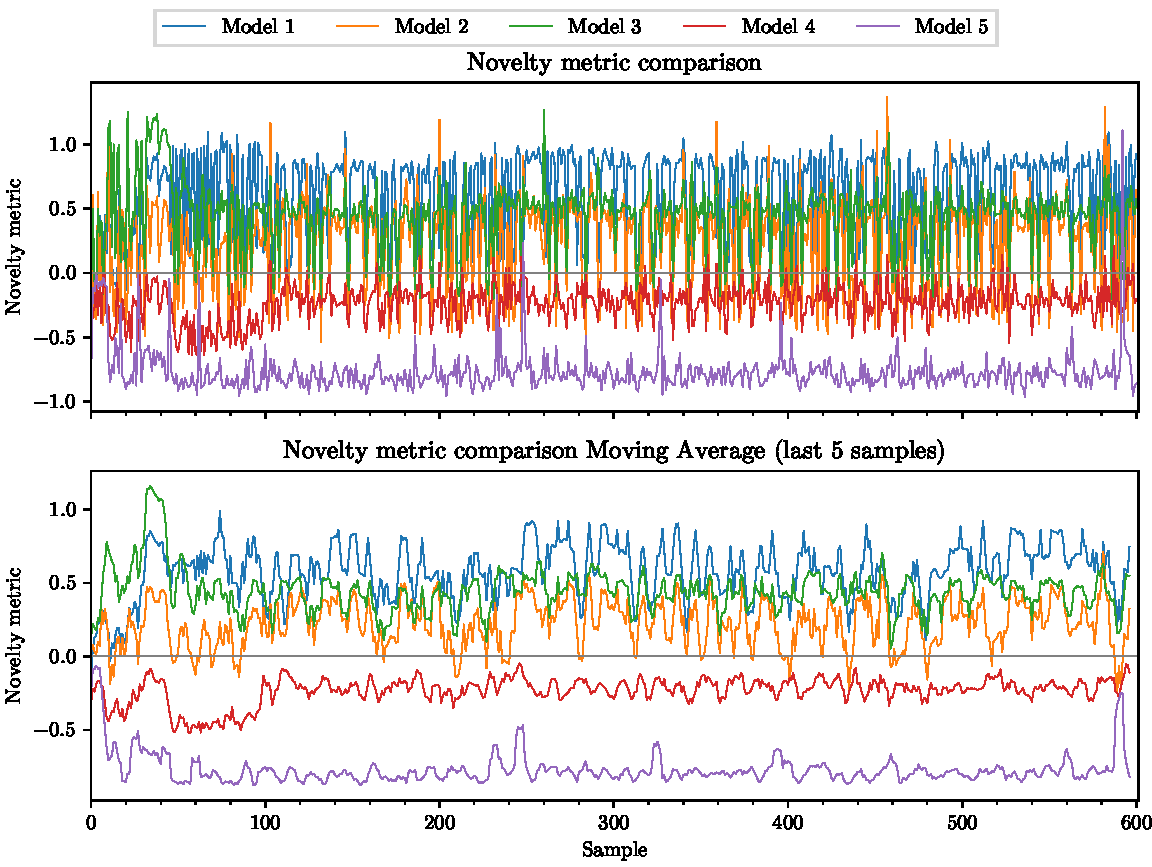
\includegraphics[angle=-90,origin=c]{images/LinearMotor/Testing.pdf}
    \caption{Novelty detection on profile 2.}
    \label{fig:axis_testing}
\end{figure}
\clearpage


\subsection{Feature scaling}
To address the problem of the non-significative features, a feature scaling method is proposed. The idea is to scale the features in such a way that the most significant features will have a higher weight in the model. To do that, a naive approach could be to visually select the important features (by eye it's evident that are the first few) and apply a small scaling factor to the others. 

This approach goes against the principle of the framework being fully automatic to train. To address this problem, an unsupervised and automatic method is proposed. The idea is to scale the features in such a way that the most significant features will have a higher weight in the model. To do that, it's possible to exploit the fact that, at this point, the K-means model is already trained and the training procedure provided labels for the dataset. It's now possible to apply a \emph{supervised} \gls{ml} algorithm in a way that is transparent to the user, so the whole procedure remains \emph{unsupervised}.

The framework is then extended to include the possibility to apply feature scaling. The two possibilities are to use the Random Forest classifier or the SelectKBest algorithm to provide the weights. Since this scaling will affect also the future snapshots, a new train of the \gls{mla} is necessary. The new model is then trained with the same training set, but with the scaled features. This approach is illustrated in \autoref{fig:scalingprocedure}.

\begin{figure}[h!]
    \centering
    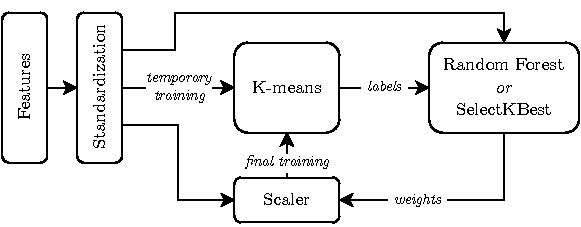
\includegraphics{images/LinearMotor/Feat_scaling.pdf}
    \caption{Feature scaling procedure.}
    \label{fig:scalingprocedure}
\end{figure}

This scaling technique is used with several configuration for both scaling the feature, and reducing the number of features, discarding the unnecessary ones. The settings of each tuned model are resumed in \autoref{tab:axis_models}. These models are describe later in this section.

\begin{table}
    \centering
    \caption{Tuned embedded models parameters}
    \label{tab:axis_models}
    \resizebox{\linewidth}{!}{%
    \begin{tabular}{ccccccccc} 
    \toprule
    \multirow{2}{*}{\textbf{Model}} & \multicolumn{2}{c}{\textbf{Feature Scaling}} & \multirow{2}{*}{\begin{tabular}[c]{@{}c@{}}\textbf{Feature}\\\textbf{Subset}\end{tabular}} & \multicolumn{4}{c}{\begin{tabular}[c]{@{}c@{}}\textbf{Training Snapshots}\\(per each profile)\\\end{tabular}} & \multirow{2}{*}{\begin{tabular}[c]{@{}c@{}}\textbf{N of}\\\textbf{clusters}\end{tabular}} \\
     & SelectKBest & Random Forest &  & 1 & 2 & 3 & 4 &  \\ 
    \hline
    Model 1 &  &  &  & 100 & 100 & 100 & 100 & 5 \\
    Model 2 &  & \checkmark &  & 100 & 100 & 100 & 100 & 3 \\
    Model 3 & \checkmark &  &  & 100 & 100 & 100 & 100 & 3 \\
    Model 4 &  & \checkmark &  & 100 & 200 & 100 & 100 & 5 \\
    Model 5 &  & \checkmark & \checkmark & 100 & 200 & 100 & 100 & 6 \\
    \bottomrule
    \end{tabular}
    }
    \end{table}

\subsubsection{Random Forest}
The Random Forest classification algorithm gives a measure of the importance of each feature, and this measure can be used to scale the features. The \gls{rf} algorithm is trained on the training set, with the labels provided by the K-means model. 

The feature importance is based on the idea that that the Gini impurity is reduced at a split in each decision tree of the forest. The more the impurity is reduced, the more important the feature used for that split is \cite{RF_featimportance}. This concept, averaged over all splits of all the trees, gives a measure of the importance of each feature.

For our purpose, the inportance is then normalized to have a maximum value of~1, so the most important feature will remain unscaled.

\subsubsection{SelectKBest}
Another tool for analyzing the importance of features is the SelectKBest algorithm. It is available in the \texttt{scikit-learn} library and is used to select the $k$ most important features or alternatively, to output a score for each feature, based on \gls{anova} statistics.

\subsubsection{Results}
scrivere qui i barplot dei pesi \todo